% --- PREAMBULO (pdflatex) ---
\documentclass[11pt, a4paper]{article}
\usepackage[a4paper, top=2.5cm, bottom=2.5cm, left=2cm, right=2cm]{geometry}
\usepackage[T1]{fontenc}
\usepackage[utf8]{inputenc}
\usepackage{lmodern}
\usepackage{amsmath}
\usepackage{array}
\usepackage{booktabs}
\usepackage{xcolor}
\usepackage{graphicx}
\graphicspath{{./}}
\usepackage{fancyhdr}
\usepackage{titlesec}
\usepackage{lastpage}
\usepackage[section]{placeins}
\usepackage[hidelinks]{hyperref}
\usepackage[spanish, es-tabla]{babel}

\usepackage{enumitem}
\setlist[itemize]{label=-}

% Paleta
\definecolor{primary}{HTML}{0F172A}
\definecolor{alertred}{HTML}{DC2626}
\definecolor{accentgreen}{HTML}{0F766E}
\definecolor{warnamber}{HTML}{D97706}
\definecolor{lightgray}{HTML}{F8FAFC}
\definecolor{darkgray}{HTML}{475569}
\definecolor{markred}{HTML}{FEE2E2}
\definecolor{markgreen}{HTML}{D1FAE5}
\definecolor{markamber}{HTML}{FEF3C7}

\newcommand{\mR}[1]{{\setlength{\fboxsep}{1.5pt}\colorbox{markred}{\textbf{#1}}}}
\newcommand{\mG}[1]{{\setlength{\fboxsep}{1.5pt}\colorbox{markgreen}{\textbf{#1}}}}
\newcommand{\mA}[1]{{\setlength{\fboxsep}{1.5pt}\colorbox{markamber}{\textbf{#1}}}}

\newcommand{\alertbox}[2]{%
  \noindent\colorbox{lightgray}{%
    \parbox{\dimexpr\textwidth-2\fboxsep\relax}{%
      \raggedright\smallskip
      \textbf{\color{alertred}{#1}}\par\smallskip
      \small #2\par\smallskip}}%
  \par\vspace{3mm}}
\newcommand{\successbox}[2]{%
  \noindent\colorbox{lightgray}{%
    \parbox{\dimexpr\textwidth-2\fboxsep\relax}{%
      \raggedright\smallskip
      \textbf{\color{accentgreen}{#1}}\par\smallskip
      \small #2\par\smallskip}}%
  \par\vspace{3mm}}

\setlength{\parindent}{0pt}
\setlength{\parskip}{6pt}

\pagestyle{fancy}
\fancyhf{}
\renewcommand{\headrulewidth}{0.4pt}
\renewcommand{\footrulewidth}{0.4pt}
\fancyhead[L]{\small\color{darkgray}\textsc{Chaco For Ever} $\bullet$ Scouting Pre-Partido}
\fancyhead[R]{\small\color{darkgray}vs San Telmo $\bullet$ Fecha 20}
\fancyfoot[L]{\footnotesize\color{darkgray}Confidencial $\bullet$ Uso interno del Cuerpo Técnico}
\fancyfoot[R]{\footnotesize\color{darkgray}Página \thepage\ de \pageref{LastPage}}

\titleformat{\section}{\normalfont\Large\bfseries\color{primary}}{\thesection}{0.6em}{}[\vspace{-2mm}\noindent{\color{accentgreen}\rule{\textwidth}{1.2pt}}]
\titlespacing*{\section}{0pt}{4mm}{4mm}
\titleformat{\subsection}{\normalfont\large\bfseries\color{darkgray}}{\thesubsection}{0.6em}{}
\titlespacing*{\subsection}{0pt}{3mm}{2mm}

\hypersetup{pdftitle={Scouting Pre-Partido - Chaco For Ever vs San Telmo},
  pdfauthor={Departamento de Big Data \& Análisis Táctico}}

\begin{document}

% --- HEADER ---
\begin{center}
  \colorbox{primary}{%
    \parbox{\dimexpr\textwidth-2\fboxsep\relax}{%
      \vspace{4mm}\centering\color{white}
      \textsc{\Large Chaco For Ever} \\ \vspace{1mm}
      \textbf{\Large SCOUTING PRE-PARTIDO} \\ \vspace{1mm}
      \small Próximo rival: San Telmo (de visitante) $\bullet$ Fecha 20 $\bullet$ Temporada 2026
      \vspace{4mm}}}
\end{center}
\vspace{3mm}

\begin{tabular}{ll}
  \textbf{Destinatarios:} & Cuerpo Técnico, Comisión Directiva \\
  \textbf{Creadores:} & Cordeiro Mariano Angel y Casco Tobias \\
  \textbf{Contacto:} & cordeiromariano17@gmail.com \\
  \textbf{Partido:} & San Telmo (local) vs Chaco For Ever (visitante) \\
  \textbf{Estado:} & Sin jugarse — análisis sobre los 19 partidos de San Telmo en 2026 \\
  \textbf{Alcance:} & Datos de la temporada 2026 (Primera Nacional) \\
\end{tabular}
\vspace{3mm}
\hrule
\vspace{3mm}

% --- 1. RESUMEN ---
\section*{1. Resumen y Plan de Partido}

Visitamos a San Telmo en un momento inmejorable: \mR{llega sin su goleador}. M. L. Batallini —autor de 4 de sus goles y único 9 de referencia en su once tipo— fue expulsado en la última fecha y no juega. A un equipo que ya generaba poco le sacan su principal vía de gol. Sumado a eso, San Telmo no es fuerte en su cancha (1.40 puntos por partido de local) y muestra grietas defensivas claras. Mostraremos una postura para ganar el partido aunque queda a criterio del entrenador.

\alertbox{Las tres claves del partido}{
  1. San Telmo de local rinde \mR{1.40 puntos} (4V-2E-4D) y recibe 10 goles en su propia cancha. No es un fortín, y sin Batallini su ataque queda diezmado. \\[1mm]
  2. Concede más de lo que genera y solo el arquero lo salva (\mR{1.30 de xG en contra} y apenas 0.95 goles recibidos). Con volumen y eficacia, el gol llega. \\[1mm]
  3. Regala penales: \mR{6 goles recibidos} por esa vía, más tres defensores a una amarilla de la suspensión. Atacar el área es la vía directa para lastimarlo.
}

\begin{table}[h!]
  \centering
  \caption{San Telmo en 2026 — local vs visitante}
  \vspace{2mm}
  \begin{tabular}{lll}
    \toprule
    \textbf{Métrica} & \textbf{De local} & \textbf{De visitante} \\
    \midrule
    Récord (9-10 pj) & \mA{4V - 2E - 4D} & 0V - 6E - 3D \\
    Puntos por partido & \mA{1.40} & 0.67 \\
    Goles a favor / en contra & \mA{10 / 10} & 5 / 8 \\
    \bottomrule
  \end{tabular}
\end{table}

Nos toca su versión de local, la columna ámbar. Es su mejor cara, pero es apenas correcta: gana menos de la mitad de sus partidos en casa y recibe un gol por partido.

\begin{figure}[htbp]
  \centering
  \fbox{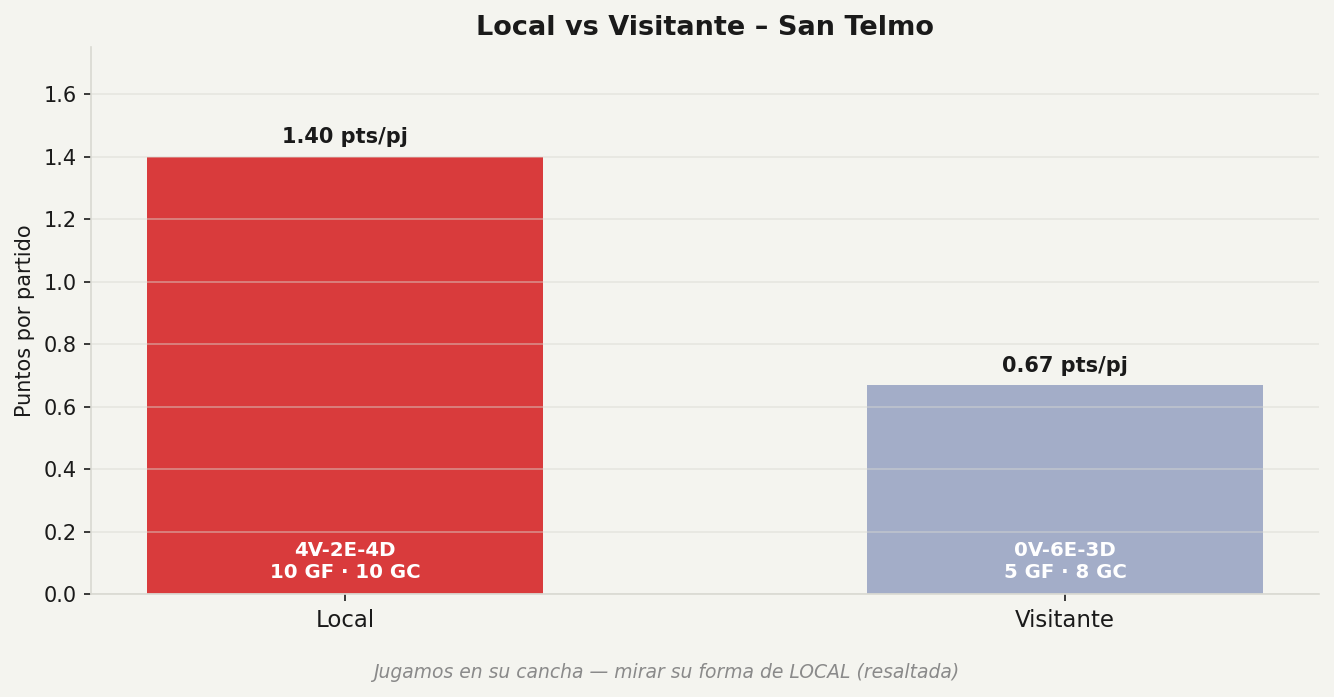
\includegraphics[width=0.80\textwidth]{local_visitante_rival.png}}
  \caption{Rendimiento de San Telmo según la cancha. La columna roja (local) es la que nos toca enfrentar: correcta, no dominante, y con 10 goles recibidos en su casa.}
\end{figure}

% --- 2. COMO LLEGA ---
\section*{2. Cómo Llega San Telmo}

La temporada de San Telmo fue un despelote institucional: \mA{tres cambios de técnico} en el año (Bianco, Perugini y Sergio Marcelo Vázquez, con Vázquez de vuelta en el banco desde junio). Esa inestabilidad se nota en la forma, cargada de empates y derrotas, con muy pocas victorias seguidas. Es un equipo sin identidad asentada.

En el mano a mano estadístico somos casi un espejo: posesión pareja, goles y xG casi calcados (0.79 vs 0.74 en goles, 0.82 vs 0.81 en xG), remates similares. Ninguno domina con claridad en el promedio. La diferencia, entonces, no está en el volumen sino en dónde cada uno es frágil, y ahí San Telmo pierde por atrás.

\begin{figure}[htbp]
  \centering
  \fbox{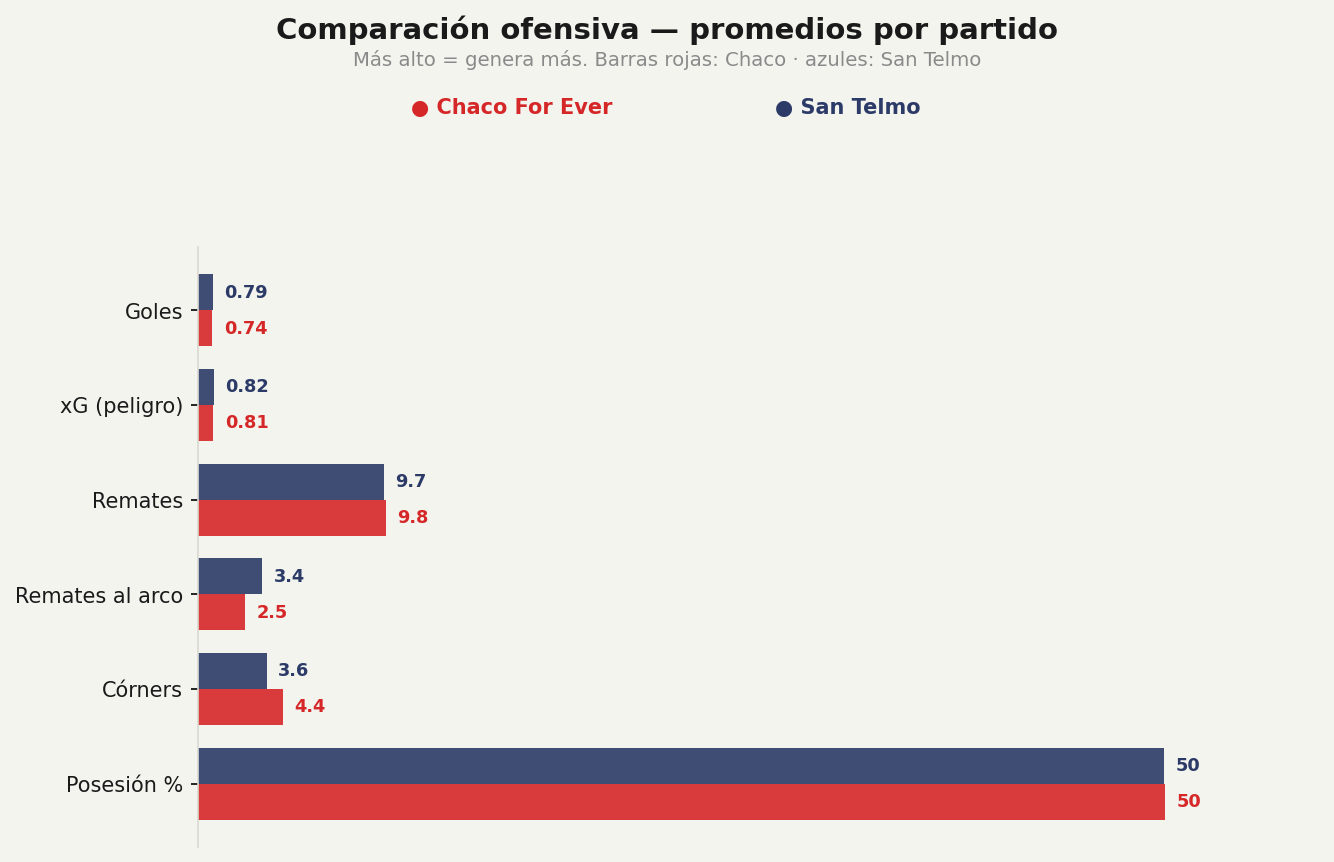
\includegraphics[width=0.8\textwidth]{comparacion_ofensiva.png}}
  \caption{Comparación ofensiva, promedios por partido. Perfiles espejo: los dos generan casi lo mismo. El partido no se define por quién genera más, sino por quién falla menos atrás.}
\end{figure}

% --- 3. SU EQUIPO ---
\section*{3. Su Equipo}

La fuerza de San Telmo pasa por un solo nombre: el arquero \mA{J. Enrico} (7.24 de promedio, jugó los 19 partidos), el que de verdad los sostiene. Su defensa aparece como la unidad más puntuada —R. Gamarra (7.13), L. Pollacchi (6.91), F. Roncaglia (6.88) y J. Motroni (6.83)—, pero conviene no leer ese puntaje como solidez: premia el volumen de despejes y cortes de una línea que vive bajo asedio, no que concedan poco. Como se ve en la sección siguiente, la defensa filtra muchas chances y es Enrico quien las tapa. Individualmente sí hay que respetar a \mA{Pollacchi} en el duelo y el juego aéreo, pero es una fortaleza personal, no del bloque.

Arriba, en cambio, dependían de un solo nombre —Batallini— y esta fecha no lo tienen. El peligro ofensivo que les queda pasa por \mA{J. González}, un atacante de mucha gambeta pero sin el gol del que se pierde el partido.

\begin{figure}[htbp]
  \centering
  \fbox{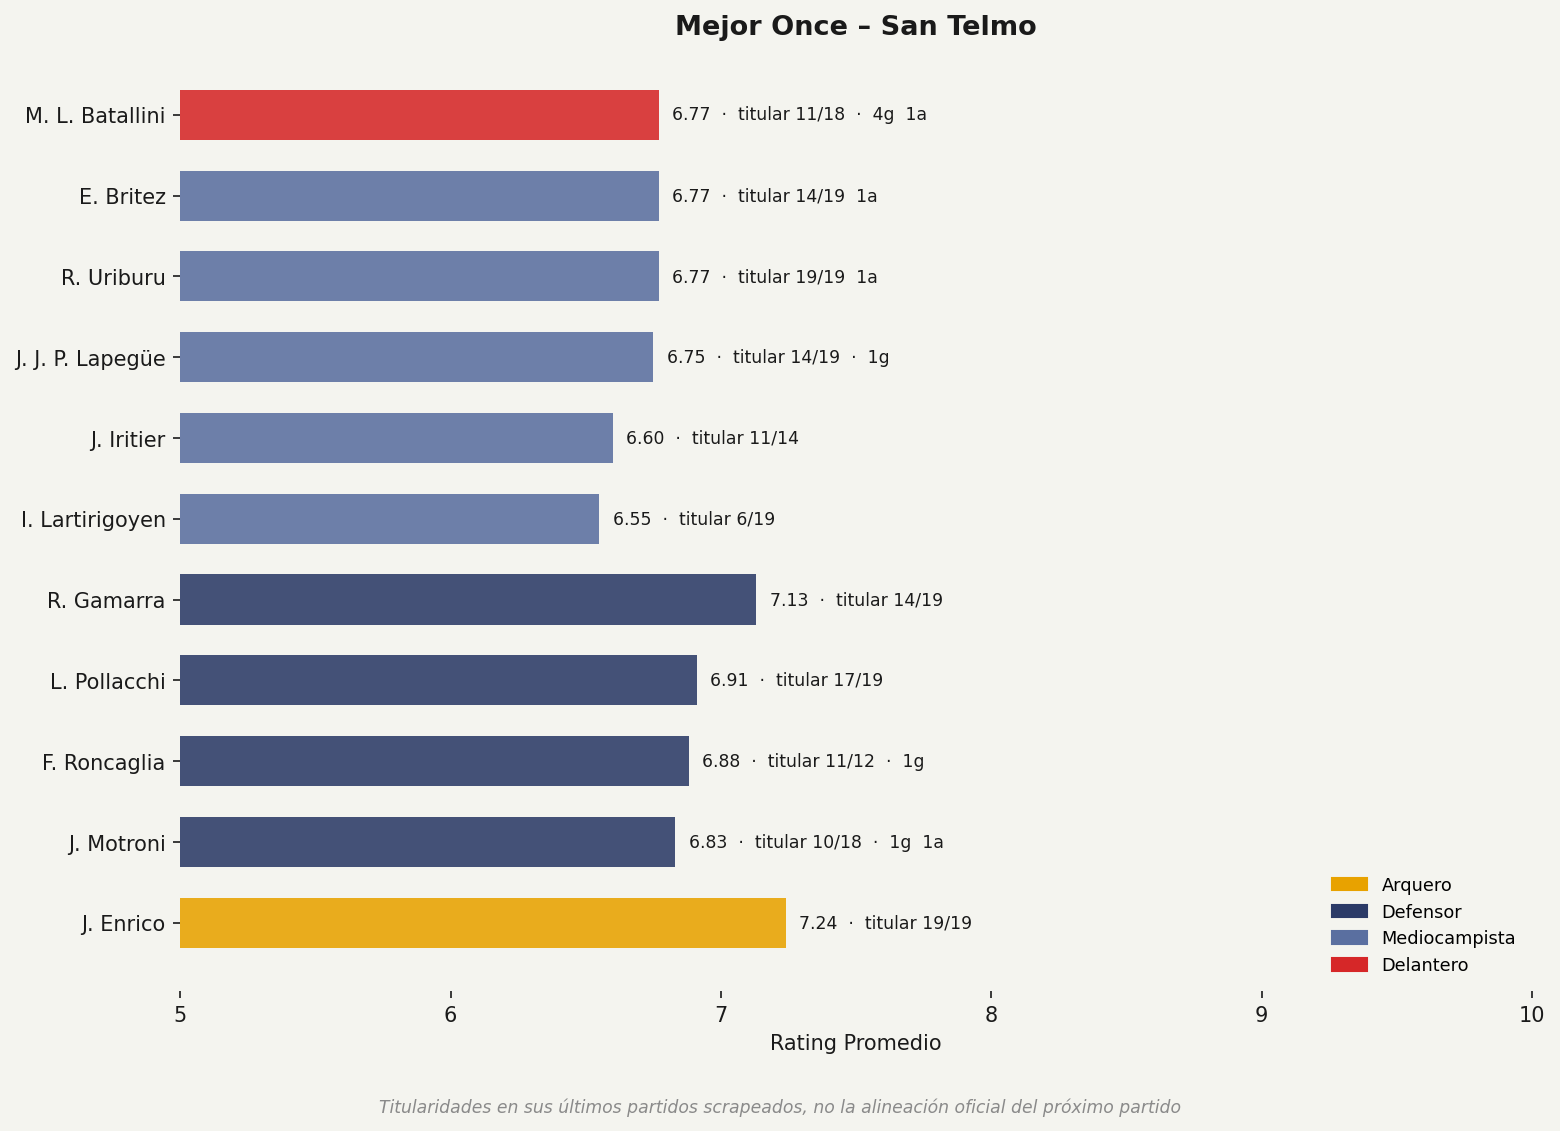
\includegraphics[width=0.72\textwidth]{mejor_once_rival.png}}
  \caption{Once más repetido de San Telmo. Su columna vertebral es defensiva. Batallini (el delantero rojo) no estará por suspensión.}
\end{figure}

\subsection*{Las formaciones de Vázquez}

El DT actual, Sergio Marcelo Vázquez, tiene un dibujo de cabecera: el \mA{4-2-3-1}, que usó en 5 partidos y en las dos últimas fechas seguidas. Su alternativa es el 4-3-1-2. El menú de toda la temporada incluyó además 4-4-2, 4-3-3 y 4-1-4-1 con distintos técnicos.

Un dato para tener presente: cuando nos visitaron en la ida salieron con un 5-4-1 ultradefensivo, pero era con técnico interino. Ahora, de local y con Vázquez, van a proponer más —esperá un 4-2-3-1 con un solo 9—, y eso, paradójicamente, nos deja más espacios para lastimar en transición.

\begin{figure}[htbp]
  \centering
  \fbox{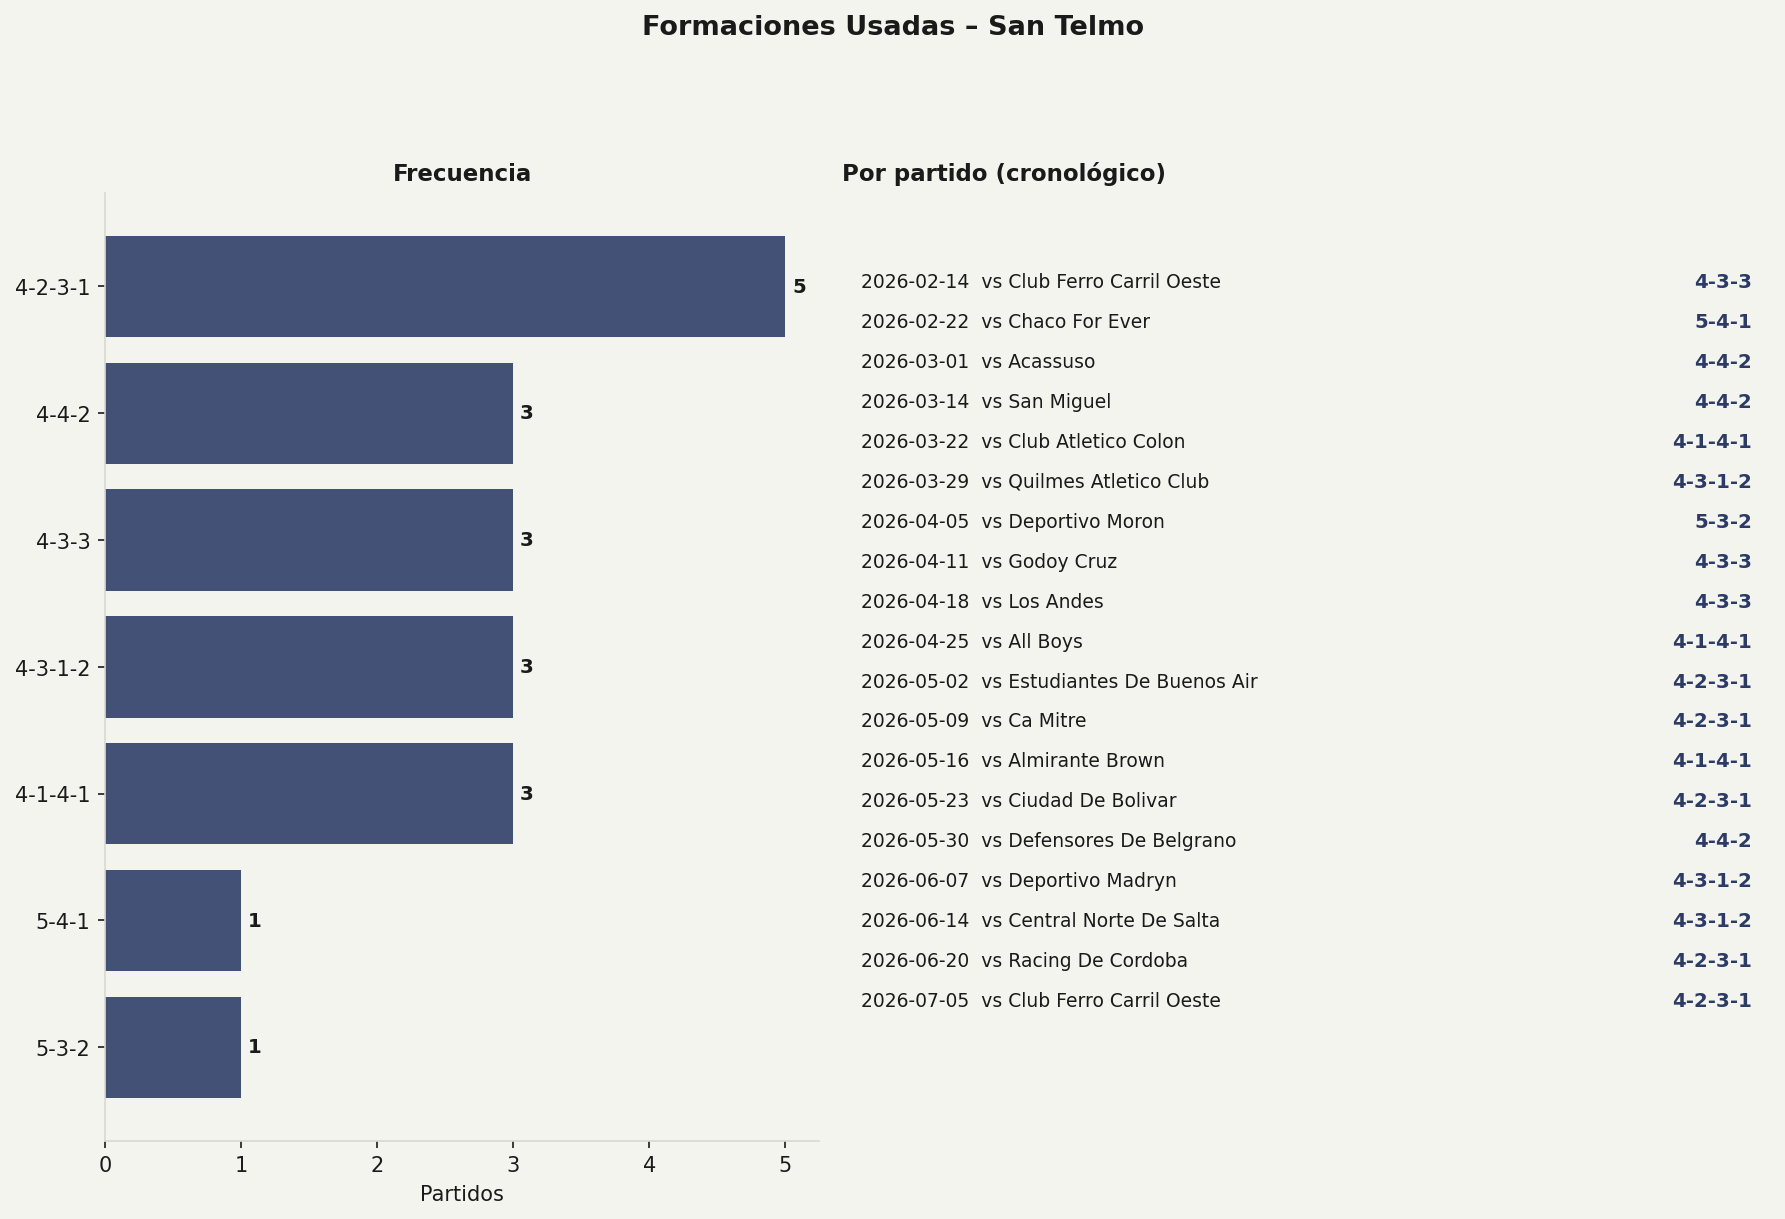
\includegraphics[width=0.92\textwidth]{formaciones_rival.png}}
  \caption{Formaciones usadas fecha a fecha. El 4-2-3-1 es la base de Vázquez y su tendencia reciente.}
\end{figure}

% --- 4. ATAQUE Y DEFENSA ---
\section*{4. Cómo Ataca y Dónde Sufre}

El ataque de San Telmo es leíble: \mA{39.6\% de entropía}, con el 60\% de sus remates naciendo del centro del área. Poca variación y, ahora, sin su definidor. Si le cerramos el carril central y marcamos de cerca a González, se queda sin ideas.

Atrás está su verdadera grieta. Concede \mR{1.30 de xG por partido} —más de lo que genera— y lo superan en tiros casi todas las fechas; que reciba apenas 0.95 goles se explica por el gran nivel de su arquero, no por su defensa. Es un rendimiento que tiende a corregirse: con volumen de situaciones claras, el gol aparece. Y hay una vía todavía más directa: el penal. San Telmo recibió \mR{6 goles de penal} en la temporada (5.3 de xG en contra por esa jugada). Defienden el área a los manotazos.

\begin{figure}[htbp]
  \centering
  \fbox{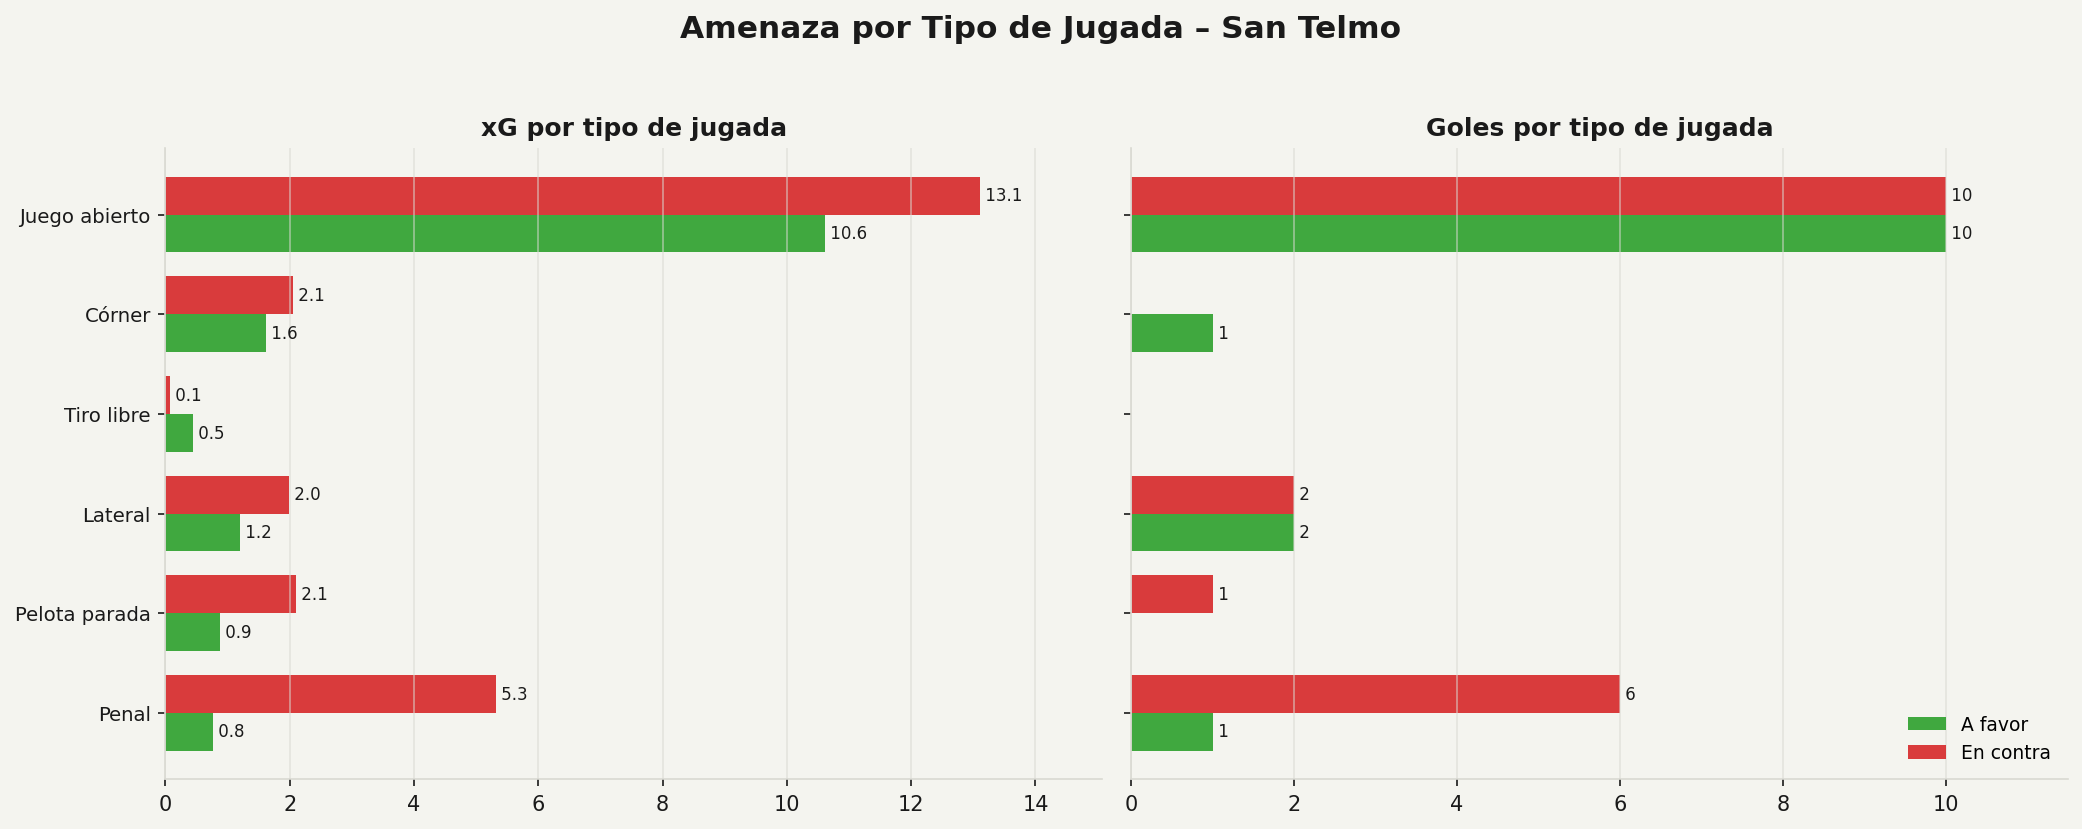
\includegraphics[width=1\textwidth]{amenaza_rival.png}}
  \caption{xG y goles de San Telmo por tipo de jugada. Genera poco en ataque y sufre en juego abierto y, sobre todo, en el penal (6 goles recibidos).}
\end{figure}

\begin{figure}[htbp]
  \centering
  \fbox{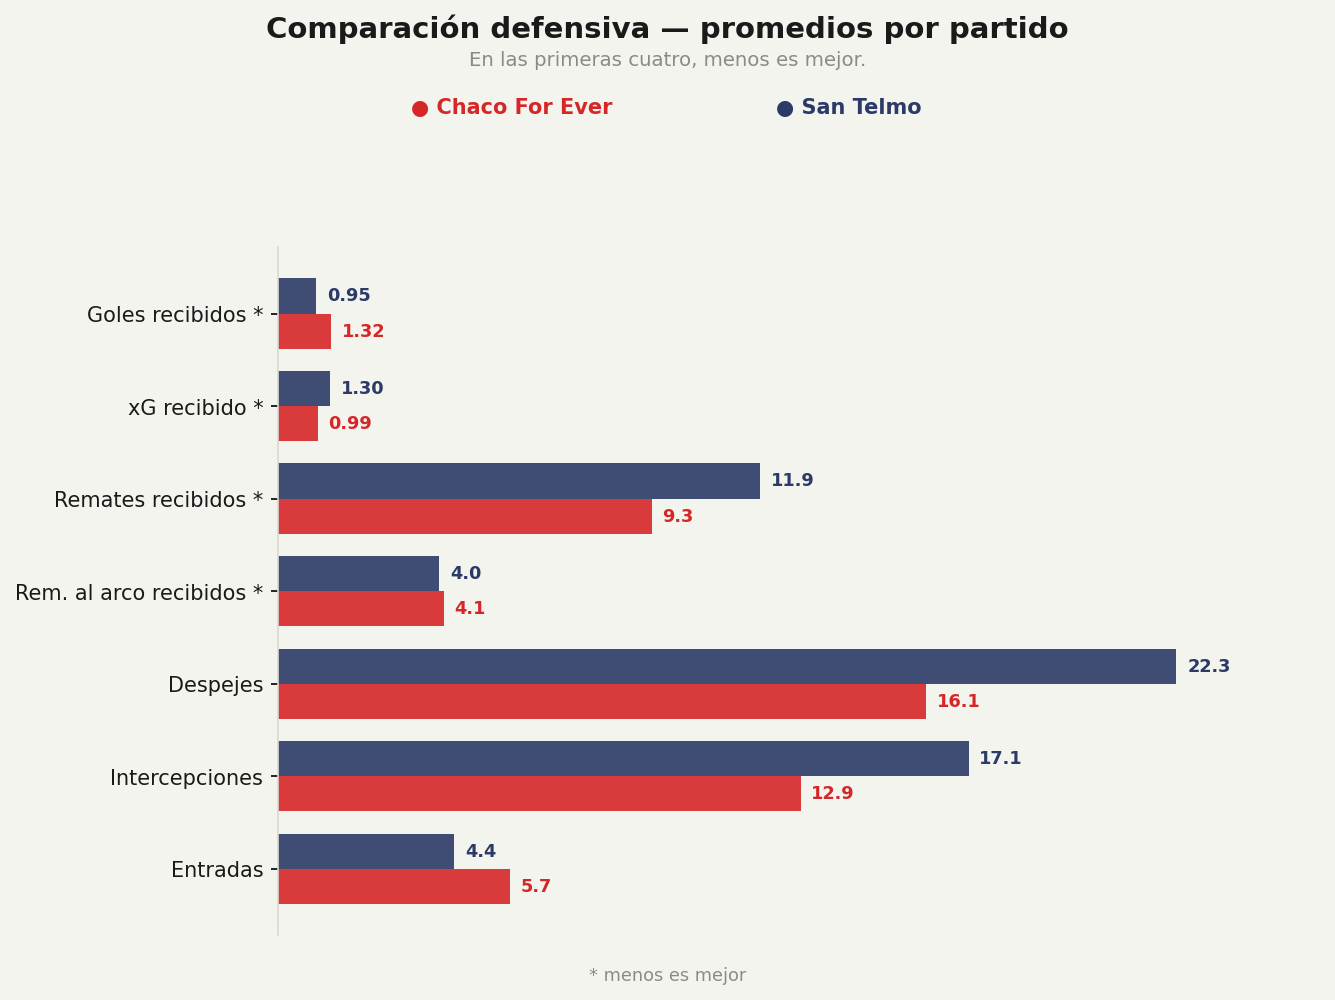
\includegraphics[width=0.78\textwidth]{comparacion_defensiva.png}}
  \caption{Comparación defensiva. San Telmo permite más remates y más xG que nosotros; solo el arquero disimula ese déficit. Defiende replegado, a base de despejes e intercepciones.}
\end{figure}

\begin{figure}[htbp]
  \centering
  \fbox{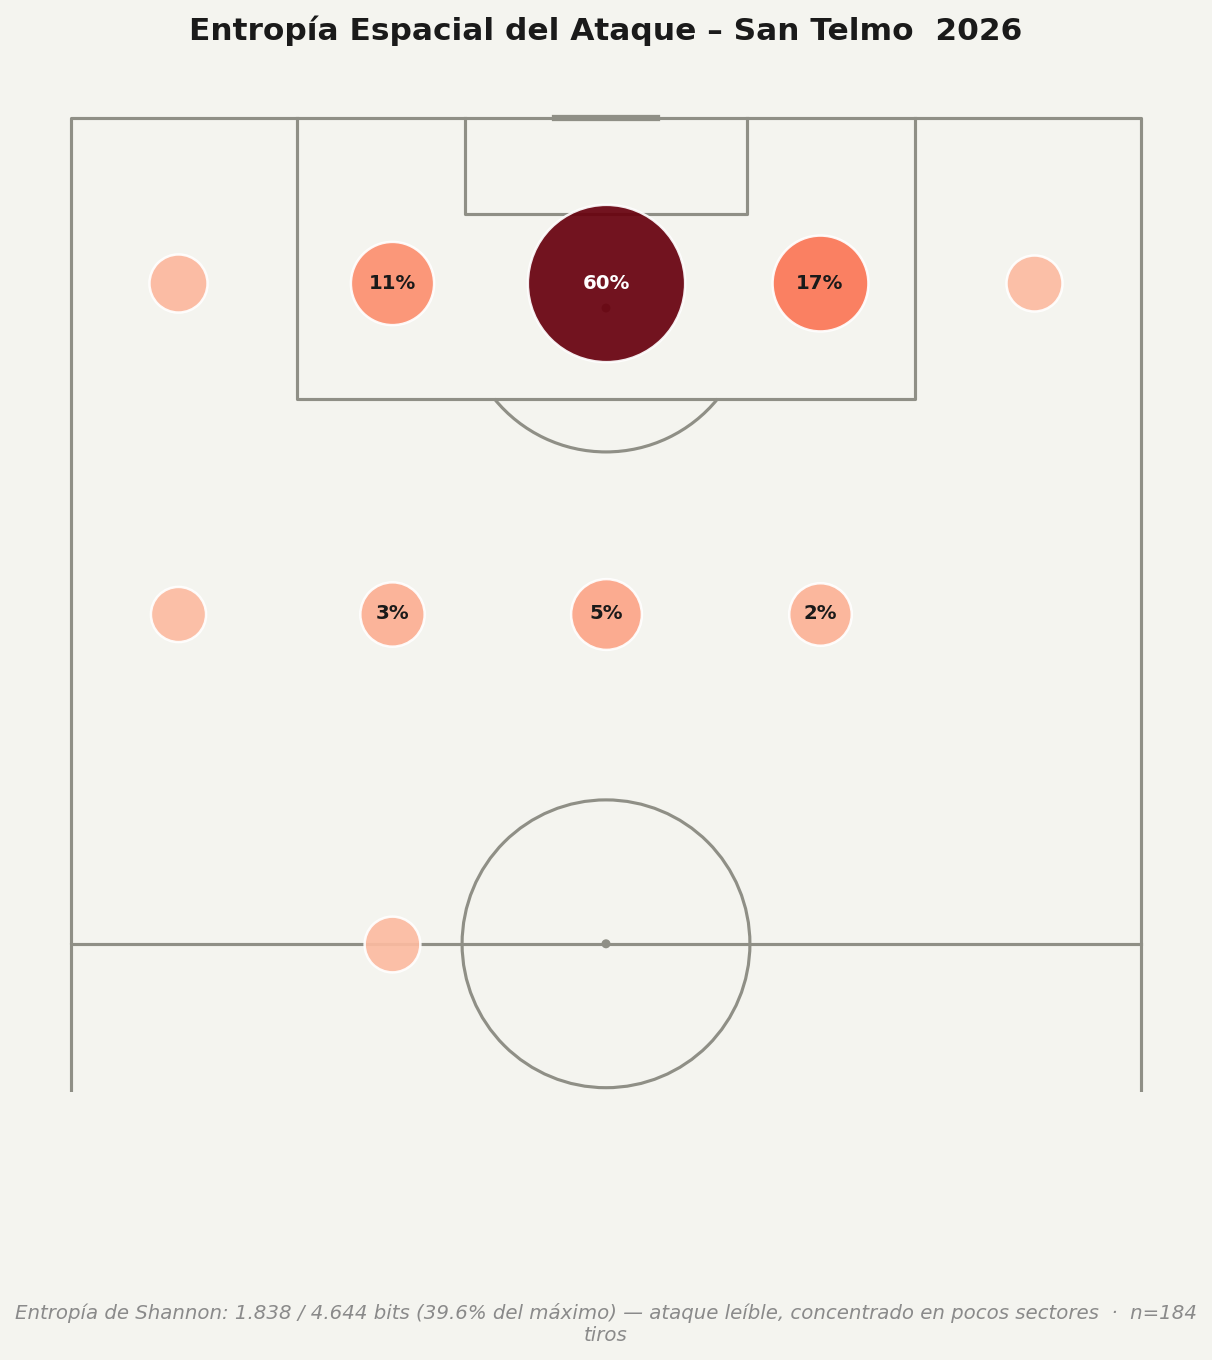
\includegraphics[width=0.55\textwidth]{entropia_rival.png}}
  \caption{Origen de los disparos de San Telmo. La concentración en el centro del área confirma un ataque predecible.}
\end{figure}

% --- 5. DUELOS INDIVIDUALES ---
\section*{5. Duelos Individuales}

Cruzamos a nuestros jugadores contra sus referentes para ver dónde ganamos y dónde hay que tener cuidado. La conclusión es consistente con todo lo anterior: \textbf{sus fortalezas individuales están atrás; nuestras ventajas, en la creación y el gol}.

\subsection*{Valdez vs Pollacchi}

Pollacchi es su defensor más duro: gana despejes, duelos e intercepciones por lejos. De igual a igual por arriba, gana él. La forma de neutralizarlo es sacarlo de su zona: Valdez le gana en toques, pases precisos, pases clave y gambeta, así que hay que llevar el duelo al pie y al espacio, no al choque.

\begin{figure}[htbp]
  \centering
  \fbox{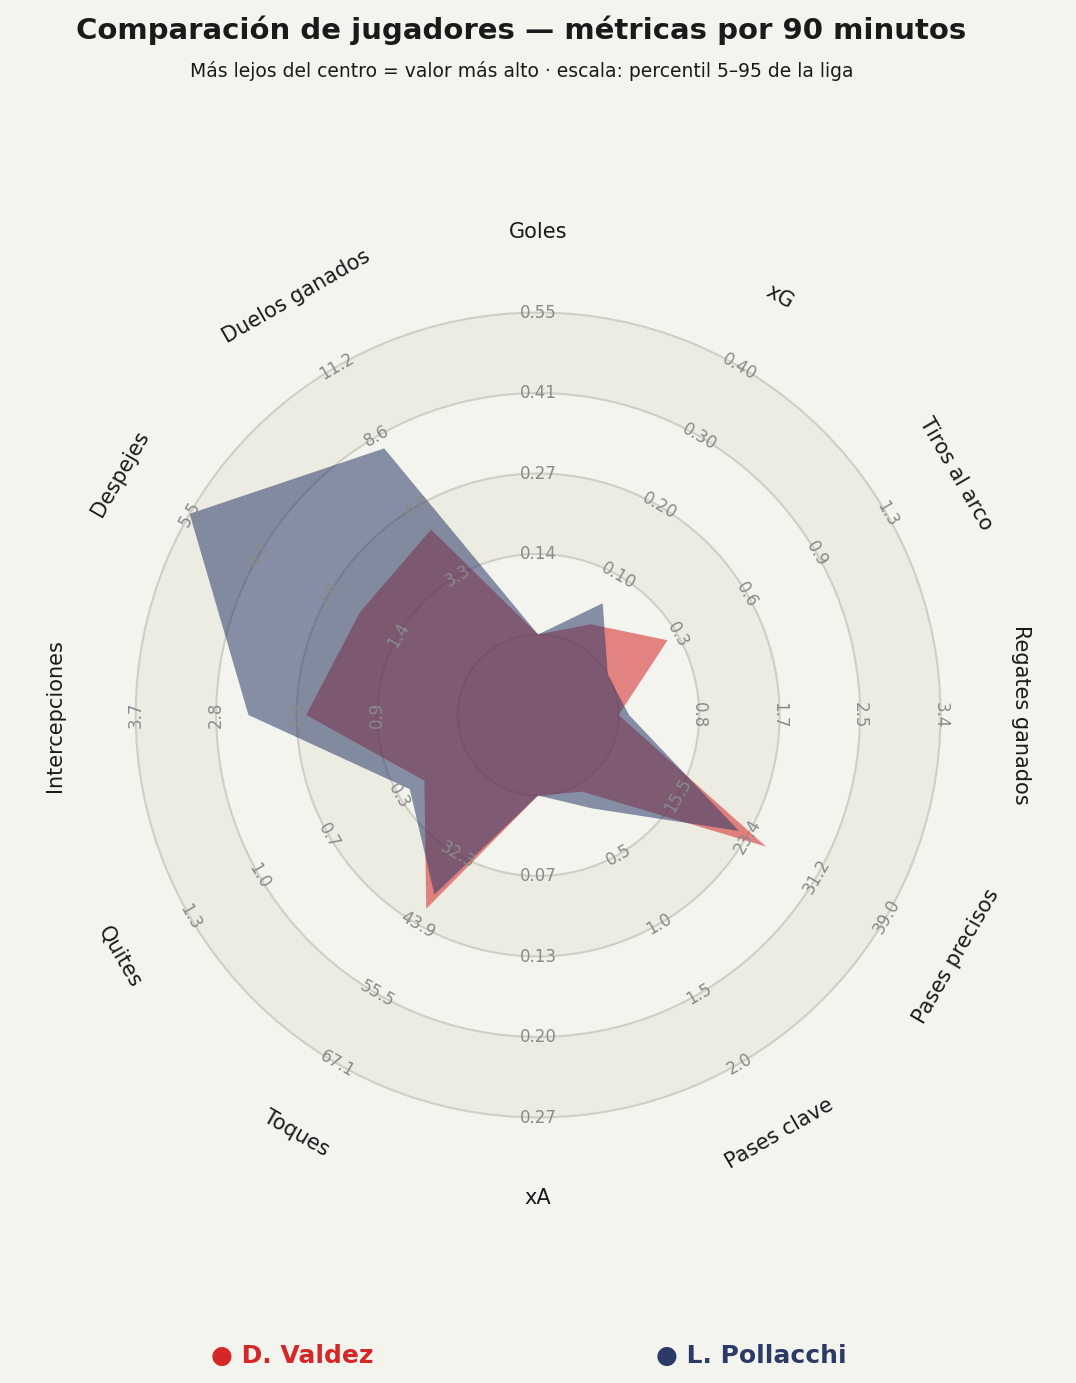
\includegraphics[width=0.62\textwidth]{Valdez_vs_Pollacchi.png}}
  \caption{Valdez (nosotros) vs Pollacchi (ellos). Él domina el juego aéreo y el duelo; nosotros, la pelota.}
\end{figure}

\subsection*{Garay vs Britez}

Perfil parecido: Britez es otro central metido, fuerte en el duelo y con volumen de pase. Pero es \mR{uno de los tres a una amarilla de la suspensión}. Atacarlo en velocidad lo obliga a elegir entre la falta —con riesgo de amarilla— o dejar pasar. Lo condiciona todo el partido.

\begin{figure}[htbp]
  \centering
  \fbox{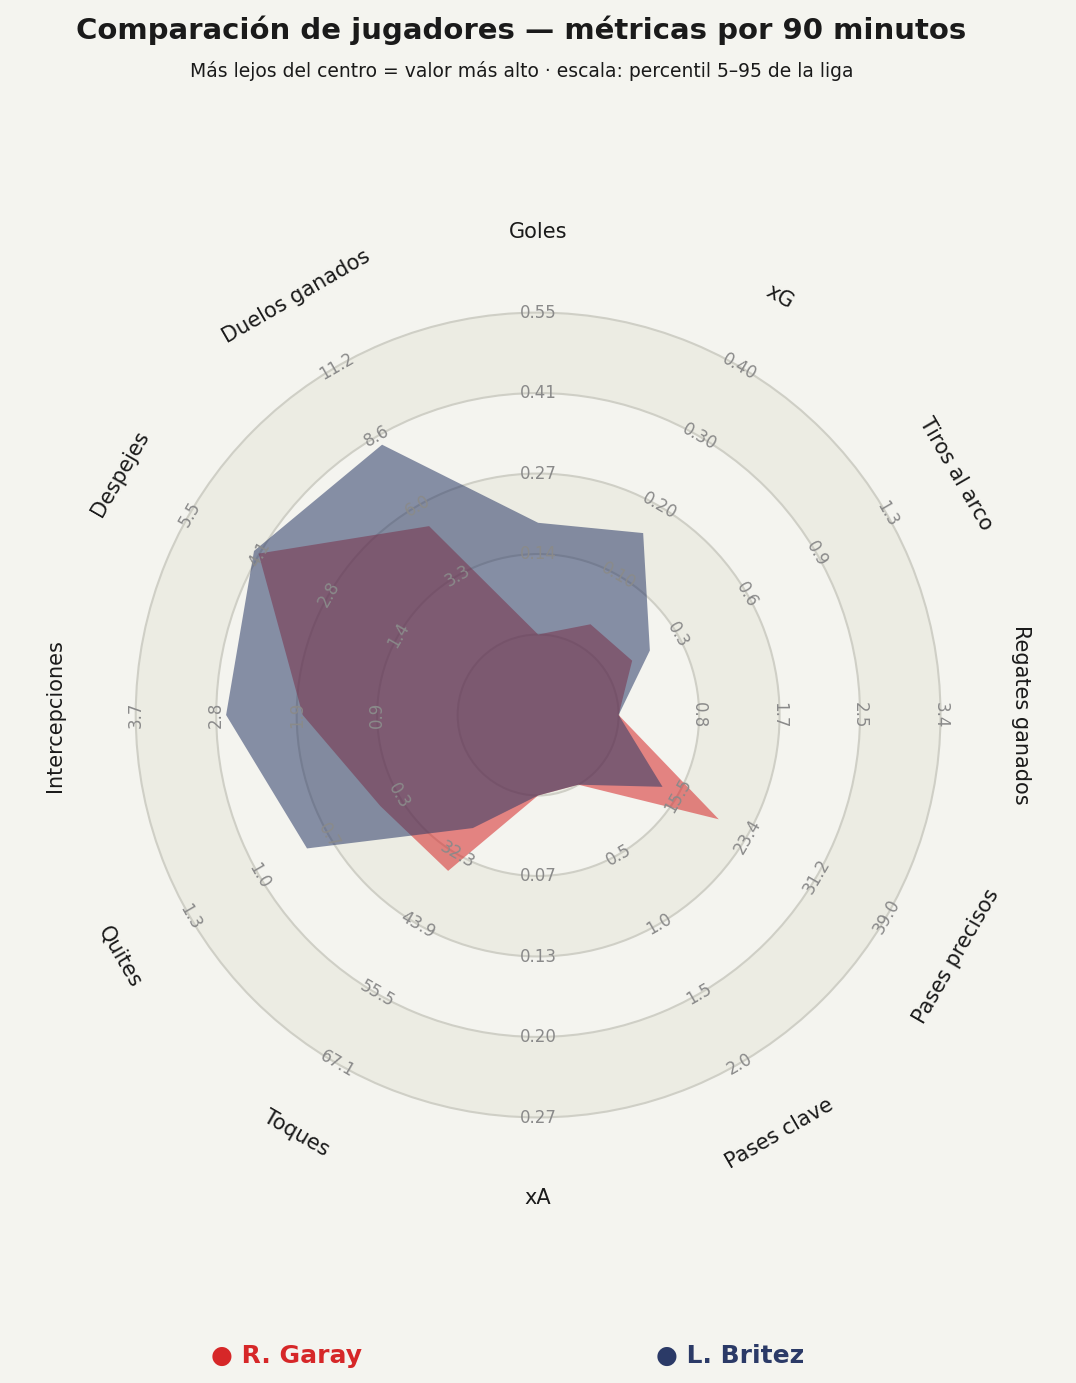
\includegraphics[width=0.62\textwidth]{Garay_vs_Britez.png}}
  \caption{Garay (nosotros) vs Britez (ellos). Defensor sólido, pero amonestado y presionable.}
\end{figure}

\subsection*{Gaggi vs González}

Acá está el jugador a vigilar: sin Batallini, \mA{González es su principal amenaza}. Encara mucho (de los mejores de la liga en regates ganados) y mete goles. Pero es gambeta, no definición de área: marca cercana, no dejarlo enganchar hacia adentro y llevarlo a la banda. Gaggi le responde con más gol, pases clave y xA, y es de los nuestros que puede desnivelar.

\begin{figure}[htbp]
  \centering
  \fbox{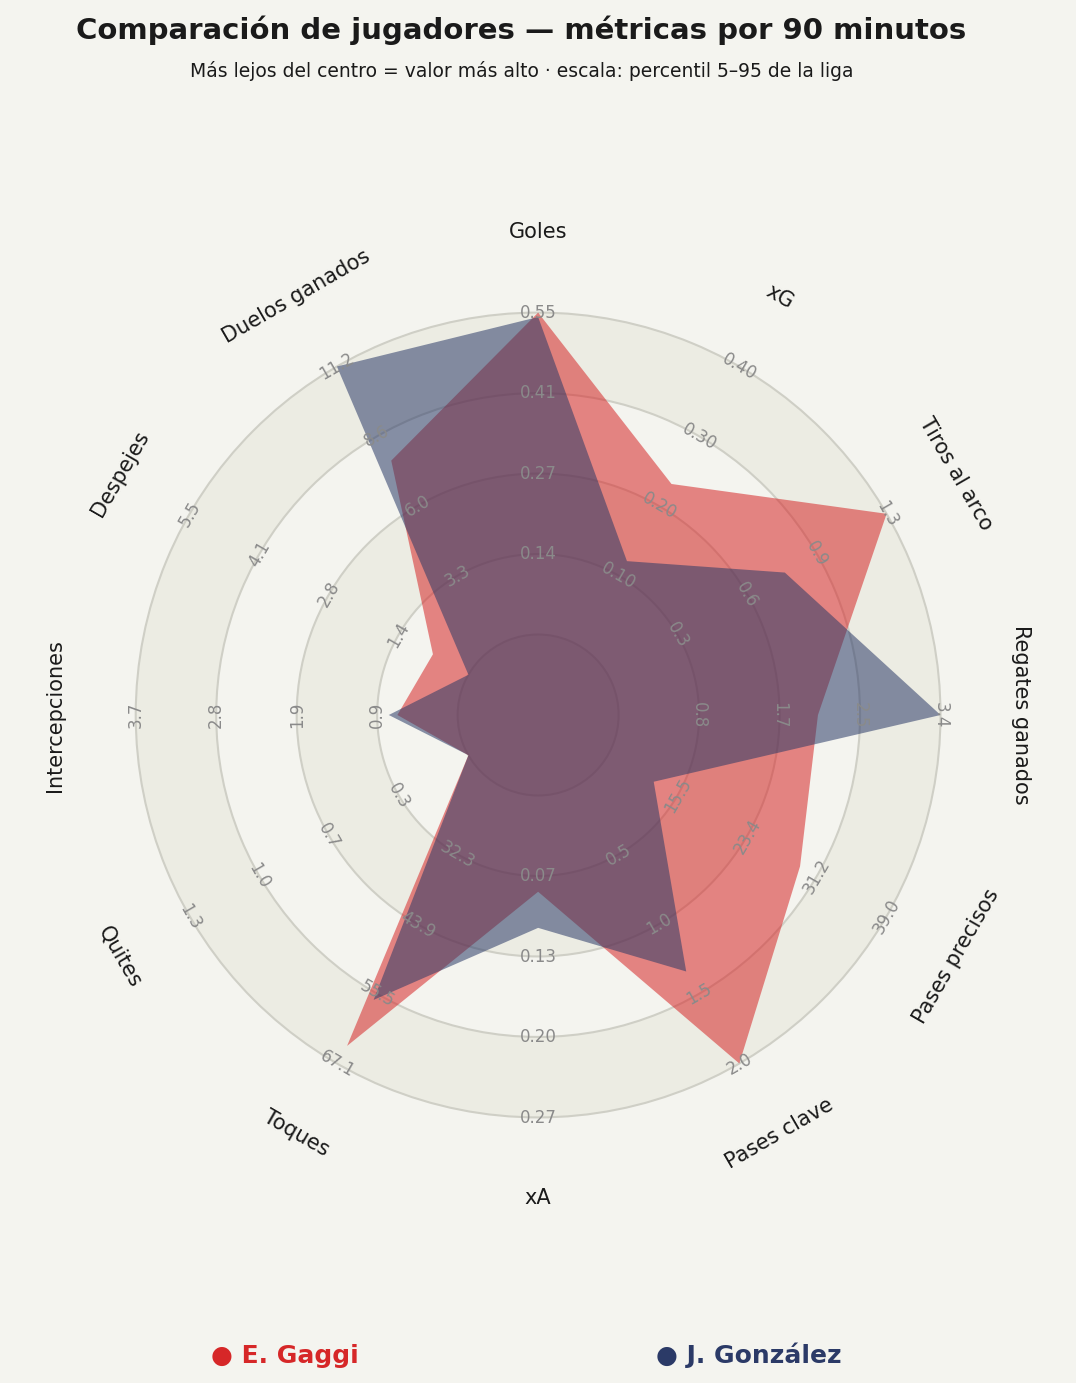
\includegraphics[width=0.62\textwidth]{radar_jugadores_cruzado.png}}
  \caption{Gaggi (nosotros) vs González (ellos). Su vía de peligro que queda tras la baja de Batallini.}
\end{figure}

% --- 6. DISCIPLINA ---
\section*{6. Disciplina}

San Telmo llega al partido con el plantel al límite. Además de la baja de Batallini por expulsión, tiene \mR{tres jugadores a una amarilla de la suspensión}: Britez, Motroni y Henríquez, dos de ellos de la línea de fondo. Es un equipo que defiende con faltas y está expuesto: cada avance en velocidad sobre esa zona los pone ante la disyuntiva de arriesgar la amarilla.

% --- 7. HISTORIAL Y ULTIMO CRUCE ---
\section*{7. Historial y Último Cruce}

El historial está parejo: tres partidos, 1V-1E-1D para Chaco, 5 goles a favor y 4 en contra. En la ida de esta temporada empatamos \mA{2-2} de local, pero el partido dejó una señal fuerte: lo \mG{dominamos por completo} y no lo ganamos. Tuvimos 55\% de la pelota, \mG{2.37 de xG contra 0.83}, 16 remates a 7, 10 córners a 5, y encima ellos terminaron con un jugador expulsado. Nos faltó una sola cosa: eficacia. Esa es, otra vez, la clave del partido.

\subsection*{Cómo evoluciona el marcador}

Modelamos con una cadena de Markov cómo se mueve el resultado de San Telmo gol a gol, y quedan dos señales que juegan a nuestro favor.

Primero, \mR{reaccionan mal cuando les convierten}: estando un gol abajo, caen a dos abajo el 60\% de las veces y solo empatan el 40\%. Es decir, si les hacemos el primer gol, tienden a hundirse más en vez de reaccionar. El primer gol vale doble: nos pone arriba y los quiebra.

Segundo, \mR{no cierran los partidos}: cuando van ganando por uno, lo dejan escapar el 38\% de las veces (3 de 8), una de ellas después del minuto 70. Aun si se ponen en ventaja, seguimos vivos. La conclusión encaja con todo lo demás: meter el primer gol es clave y, además, los rompe.

% --- 8. PLAN DE PARTIDO ---
\section*{8. Plan de Partido — Vamos a Ganarlo}

El escenario es favorable y es posible conseguir los tres puntos. El plan se apoya en cinco pilares:

\begin{itemize}
  \item \textbf{Anular a González y cerrar el centro.} Con Batallini afuera, casi todo su peligro pasa por González encarando. Marca cercana, no dejarlo enganchar hacia adentro y llevarlo a la banda. Con el carril central cerrado, su ataque leíble se queda sin vías.
  \item \textbf{Eficacia, la lección de la ida.} No es que no generemos: es que no convertimos. Hay que llegar con volumen y rematar claro para romper a Enrico, que viene sobre-rindiendo. Las que se generen, meterlas.
  \item \textbf{Atacar el área para forzar penal o falta.} Es su grieta más grande (6 goles recibidos de penal). Meter gente al área y buscar el desborde sube la chance de penal o de falta peligrosa. Vía directa y de bajo riesgo.
  \item \textbf{Presionar a los defensores amonestados.} Britez, Motroni y Henríquez están al borde de la suspensión. Atacarlos en velocidad los condiciona todo el partido.
  \item \textbf{No regalar el partido.} Es la única condición para que el plan funcione: no conceder el primer gol ni un penal tonto, con cabeza fría en los cruces. Con su ataque diezmado, si no les regalamos nada, les cuesta muchísimo lastimarnos.
\end{itemize}

\end{document}
